%-------------------------------------------------------------------------------
% LATEX TEMPLATE ARTIKEL
%-------------------------------------------------------------------------------
% Dit template is voor gebruik door studenten van de de bacheloropleiding 
% Informatica van de Universiteit van Amsterdam.
% Voor informatie over schrijfvaardigheden, zie 
%                               https://practicumav.nl/schrijven/index.html
%
%-------------------------------------------------------------------------------
%	PACKAGES EN DOCUMENT CONFIGURATIE
%-------------------------------------------------------------------------------

\documentclass{uva-inf-article}
\usepackage[dutch]{babel}
\usepackage{graphicx}
\usepackage{subcaption}
\usepackage{placeins}
\usepackage{amsmath}
\usepackage{caption}
\usepackage{grffile}






\usepackage[style=authoryear-comp]{biblatex}
\addbibresource{references.bib}

%-------------------------------------------------------------------------------
%	GEGEVENS VOOR IN DE TITEL, HEADER EN FOOTER
%-------------------------------------------------------------------------------

% Geef je artikel een logische titel die de inhoud dekt.
\title{Power-Performance Characterisation Report}

% Vul de naam van de opdracht in zoals gegeven door de docent en het type 
% opdracht, bijvoorbeeld 'technisch rapport' of 'essay'.
\assignment{Assignment 2}
\assignmenttype{Report}

% Vul de volledige namen van alle auteurs in en de corresponderende UvAnetID's.
\authors{Adam Rakun; Matteo D'Urso}
\uvanetids{16339908; 16349210;}

% Vul de naam van je tutor, begeleider (mentor), of docent / vakcoördinator in.
% Vermeld in ieder geval de naam van diegene die het artikel nakijkt!
\tutor{Hang Xu}
\mentor{}
\docent{Anuj Pathania}

% Vul hier de naam van je tutorgroep, werkgroep, of practicumgroep in.
\group{Group 11}

% Vul de naam van de cursus in en de cursuscode, te vinden op o.a. DataNose.
\course{Embedded Systems}
\courseid{5063EMSY6Y}

% Dit is de datum die op het document komt te staan. Standaard is dat vandaag.
\date{\today}

%-------------------------------------------------------------------------------
%	VOORPAGINA 
%-------------------------------------------------------------------------------

\begin{document}
\maketitle

%-------------------------------------------------------------------------------
%	INHOUDSOPGAVE EN ABSTRACT
%-------------------------------------------------------------------------------
% Niet toevoegen bij een kort artikel, zeg minder dan 10 pagina's!

%TC:ignore
%\tableofcontents
%\begin{abstract}
%\end{abstract}
%TC:endignore

%-------------------------------------------------------------------------------
%	INHOUD
%-------------------------------------------------------------------------------
% Hanteer bij benadering IMRAD: Introduction, Method, Results, Discussion.


\section{Introduction [0.5 Points]} 

%Give an introduction to the report, explaining what you plan to do, what results you expect, and why they are important. You must take a scientific approach to this report. Explain your hypotheses first here. Your experiments later should confirm or contradict these hypotheses.

%\par\vspace{\baselineskip}
    In this report, we perform a systematic power–performance characterization of AlexNet inference on the Khadas VIM3 platform, which features an ARM big.Little CPU architecture and a Mali GPU. The inference is executed using the Pipe-All framework, which enables flexible mapping of neural network workloads across the available processing elements. 

    Our goal is to quantify how different power-efficiency knobs (namely CPU frequency scaling, pipeline partitioning, and component ordering) affect the three primary perfomance metrics: throughput (FPS) , latency, and overall system power consumption (Watts).

More precisely, we will measure these three values while scaling CPU's frequencies and changing pipeline's partitions, so that we get the following graphs:

1. Power-Performance graphs for {\em AlexNet} on {\em Little} CPU cluster at different frequencies.

2. Power-Performance graphs for {\em AlexNet} on {\em big} CPU cluster at different frequencies.

3. Power-Performance graphs for {\em AlexNet} on {\em GPU} at different {\em big}/{\em Little} CPU frequencies.

4. Power-Performance graphs for {\em AlexNet} for different partition points, at fixed frequencies and fixed component order.

5. Power-Performance graphs for {\em AlexNet} different component orders, at fixed frequencies and fixed partition points.

\par\vspace{\baselineskip}

Before conducting the experiments, we formulate the following hypotheses for the five points above:

\begin{itemize}
    \item \textbf{H1:} Increasing the operating frequency of the Little CPU cluster will result in a gradual (quite smaller that that of the Big CPU) increase in power consumption while providing moderate performance improvements, reflecting the energy-efficient (low power, low efficiency) design of the Little cores.
    
    \item \textbf{H2:} Increasing the operating frequency of the Big CPU cluster will lead to (significantly) higher power consumption compared to the Little cluster, especially at high frequencies (because of its high power - high performance design). Throughput and latency should be improving with increasing the frequency.
    
    \item \textbf{H3:} When AlexNet is executed entirely on the GPU, variations in Big and Little CPU frequencies will still have an effect on power consumption and performance  because of the overhead (memory, synchronization, preprocessing...) carried out by the CPUs. But we expect the effect to be almost negligible. 
    
    \item \textbf{H4:} Different pipeline partition points will expose distinct power--performance trade-offs which rely on AlexNet's design.  Early convolutional layers of AlexNet are computationally intensive and well suited for GPU execution, while later layers are lighter and more appropriate for CPU execution. Assigning too few layers to the GPU is expected to underutilize its parallelism. On the other hand, assigning too many layers may underutilize the CPUs' performances. \\
    We therefore hypothesize that an intermediate partitioning, where the GPU processes early layers, the Big CPU processes intermediate layers, and the Little CPU processes final layers, will achieve the best power--performance trade-off.

    \item \textbf{H5:} Changing component orders with fixed pipeline partition points and CPU frequencies is expected to significantly affect both performance and power. Component orders that assign computationally heavier stages to faster processing elements (such as the GPU or Big CPU) earlier in the pipeline are expected to achieve higher throughput and lower latency, as this reduces the likelihood of a slow stage becoming the bottleneck. And with improving pipeline balance, those orders are also expected to be more power-efficient (as higher throughput reduces overall execution time and avoids prolonged activation of processing elements).


    
\end{itemize}

The experiments presented in this report are designed to test these hypotheses by isolating different individual system parameters (frequencies, pipeline order and partitions) while keeping all other variables constant. The resulting power--performance graphs enable a good starting insight of trends, bottlenecks, and inefficiencies, which are essential for the following design of our effective runtime Governor that aims to meet performance targets while minimizing power consumption.



\section{Experimental Setup [0.25 Points]} 

% Give an introduction to the experimental setup. This section should describe your (detailed) understanding of both the hardware {\em (Amlogic A311D HMPSoC)}, software {\em(AlexNet)}, and framework {\em(PipeAll)}. 
%\par\vspace{\baselineskip}

\textbf{Hardware Platform}

All experiments are conducted on the Khadas VIM3 development board, which is based on the Amlogic A311D heterogeneous multiprocessor system-on-chip (HMPSoC). The A311D integrates a big.Little CPU architecture consisting of four high-performance ARM Cortex-A73 cores (Big CPU) and two power-efficient ARM Cortex-A53 cores (Little CPU). The platform also includes a Mali GPU that supports general-purpose computation via OpenCL.

The heterogeneous nature of the platform enables multiple execution modes, allowing tasks to be mapped to either the Big CPU cluster, the Little CPU cluster, or the GPU, each offering different power--performance characteristics. Dynamic Voltage and Frequency Scaling (DVFS) is supported for both CPU clusters, enabling runtime adjustment of operating frequencies as a power-efficiency control knob. GPU frequency scaling, however, is not exposed on this platform.

The board is powered via an external power supply, and total system power consumption is measured at the input using an external USB power meter. This measurement includes the power consumed by all on-board components, such as the CPU clusters, GPU, memory subsystem, and cooling fan. To ensure consistency across experiments, the fan configuration is fixed throughout all measurements.

\par\vspace{\baselineskip}

\textbf{Software Workload}

The workload used in this study is AlexNet, a convolutional neural network widely used as a benchmark for image classification tasks. AlexNet consists of a sequence of convolutional, pooling, and fully connected layers, making it representative of real-world deep learning inference workloads with varying computational intensity across layers.

Performance is evaluated using two primary metrics: throughput and latency. Throughput is measured in frames per second (FPS) and indicates how many input images the system can process per second. Latency measures the average time required to process a single input frame from start to finish.

\par\vspace{\baselineskip}

\textbf{Execution Framework}

Inference execution is performed using the Pipe-All framework, which is built on top of the ARM Compute Library. Pipe-All enables the partitioning of a neural network into multiple subgraphs that can be executed concurrently on different processing elements of a heterogeneous system. Each subgraph corresponds to a pipeline stage that is mapped to either the Big CPU cluster, the Little CPU cluster, or the GPU.

The framework can divide the neural network into different pipeline stages, as well as configure a component order, which specifies the sequence in which processing elements appear in the pipeline. By adjusting these parameters, it is possible to shift computational load between processing elements and alter the pipeline bottleneck.
AlexNet has 8 partition points by which it can be divided into pipeline stages. It is not possible to divide a single layer into different stages.

%All experiments are conducted under controlled conditions by varying one parameter at a time (e.g., CPU frequency, partition points, or component order) while keeping other parameters fixed, enabling a systematic evaluation of power--performance trade-offs on the heterogeneous platform.%


\section{Methodology [0.25 Points]} 

%Describe the methodology for characterization. Elaborate what kind of measurements you take. Finally, explain how you logically organize the experiments.

%\par\vspace{\baselineskip}

For the experiments run to answer the hypotheses listed above, we used the following system setup. 

\begin{itemize}
    \item The fan of the Khadas VIM3 is set to a constant speed, to ensure that its energy consumption is constant.
    \item For each inference run, the number of frames is set to be at least 60 to get a reliable performance measurement. Numbers lower than 60 might lead to a false result as unexpected events on OS level influence execution.
    \item The power meter is read manually. To calculate the power consumption, we used the following formula:
    $ \text{W} = (\frac{x}{1000} ) / \frac{t}{3600}  $, where $x$ is the value in $mWh$ ($1 Wh = 3600 J$) which we manually read from the power meter.
    For experiments where $t$ or mWh were very small, we increased the number of frames to get more reliable measurements.
    \item The DVFS scaling of the system governor was set to manual and scripts were used to change the frequency during experiments.
    
\end{itemize}


Regarding the choice of the fixed parameters in experiments we came to the following conclusions:

\textbf{Experiments 1 and 2} have a straightforward setup. Both partition points were set to 8, to isolate the execution onto a single component. Then we ran inference for every frequency of the CPU while fixing the other CPU at its lowest frequency, in case it handled other (unrelated) tasks during execution. \\

\textbf{Experiment 3} delegates the execution entirely to the GPU in a similar fashion as in experiments 1 and 2. 
However, as the cartesian product of the possible frequencies of the little CPU and big CPU is too big, we reduced the frequencies at which a measurement is made. We only used frequencies with larger increments in between them to get the bigger picture, while keeping the sample size smaller. We believe that the overall pattern of the results can still be seen using fewer measurements and the finding remains reliable. \\

\textbf{Experiment 4} is more complicated with respect to the choice of the setup of the experiment. As the space of possible variations is too large too even getting close to covering it exhaustively, we had to make some assumptions. 
Regarding the component order, we believe that the most reasonable order is GPU -- big CPU -- little CPU, as it resembles a {\em ground truth of efficiency}. The GPU covers the most intensive and parallelizable computations. The big CPU covers computations that are less intense and the little CPU covers the least intense computations. %We expect that this setup introduces the least unexpected variance to the power-performance measurements.
For a similar reason we used frequency values of 1200 MHz for the little CPU and 1800 MHz for the big CPU. Those values are in a moderate frequency range where the CPUs operate efficiently. \\
We then ran three {\em sub-experiments} to get the trade off between all component pairs. In the first sub-experiment we fixed the size of the little CPU stage and evaluated trade-off between the big CPU and the GPU. We have done that by fixing the second partition point ($pp_2 = 6$) and iterating over through the possible positions of the first partition point ($0 \leq pp_1 \leq 6$). The second sub-experiment was similar with the first partition point $pp_1=2$ fixed and the second partition point $2 \leq pp_2 \leq 8$ variable. This fixed the the size of the GPU stage and evaluated trade-off between big CPU and little CPU. Similarly, for the last sub-experiment we fixed the big CPU stage and evaluated trade-offs between little CPU and GPU. To do that we fixed the difference between the two partition points to 3 and iterated through the possible positions of the first partition point ($0 \leq pp_1 \leq 5$).
Note: technically {\em Pipe-All} does not allow to fix a partition point on the 0th layer, however, that is semantically the same as fixing the partition point on the last layer and shifting the order. I.e. $pp_1=0, pp_2=6$ with order $G-B-L$ is the same as $pp_1=6, pp_2=8$ with order $B-L-G$ as it associates the first 6 layers with the big CPU and the last 2 with the little CPU.


\textbf{Experiment 5} is also complicated for analogous reasons of experiment 4. We chose the partition points to be $pp_1=2$, $pp_2=5$ as we wanted to get a balanced load distribution. As the first two layers are the largest, the stage is only of 2 layers. The remaining 6 layers were subdivided equally into 2 stages of 3 layers each. We chose the power frequencies of the big CPU and the little CPU to be 1800 MHz and 1200 MHz, for an analogous reason as in experiment 4. We ran all possible processor permutations as there were only 6. 

\section{Results [0.75 Points]} 

Provide your results in form of graphs (not tables). You must critically think about the important trends in your graphs and provide logical explanations.

These are the minimum results (for full sub-grades) you must provide -

1. Power-Performance graphs for {\em AlexNet} on {\em Little} CPU cluster at different frequencies.

2. Power-Performance graphs for {\em AlexNet} on {\em big} CPU cluster at different frequencies.

3. Power-Performance graphs for {\em AlexNet} on {\em GPU} at different {\em big}/{\em Little} CPU frequencies.

4. Power-Performance graphs for {\em AlexNet} for different partition points, at fixed frequencies and fixed component order.

5. Power-Performance graphs for {\em AlexNet} different component orders, at fixed frequencies and fixed partition points.

Nevertheless, there are additional (non-graded) experiments you can perform which will give your Governor design the needed edge in the competition. For example, you can repeat above experiments for not entire graph but for different layer types using {\em Pipe-All} partitioning to isolate only certain layer(s) on a given component.



\par\vspace{\baselineskip}

% ----- 1 ------
\textbf{1. Power-Performance graphs for AlexNet on Little CPU cluster at different frequencies.}\\

\par\vspace{\baselineskip}

\begin{figure}[!t]
    \centering
    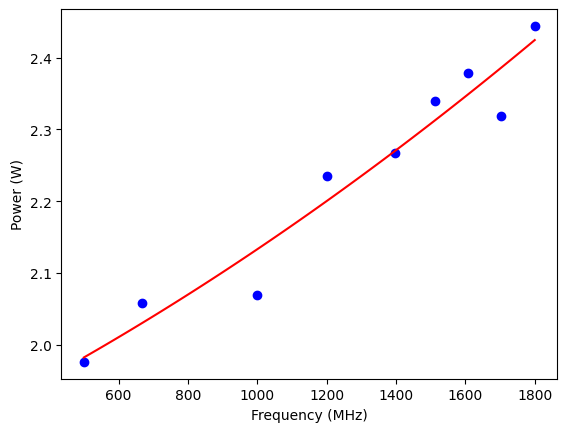
\includegraphics[width=0.85\linewidth]{figures/11.png}
    \caption{}
    \label{fig:exp1-little-freq_power}
\end{figure}

As the Little CPU frequency increases, the measured system power rises gradually and is well-approximated by an almost linear trend.


\begin{figure}[!t]
    \centering
    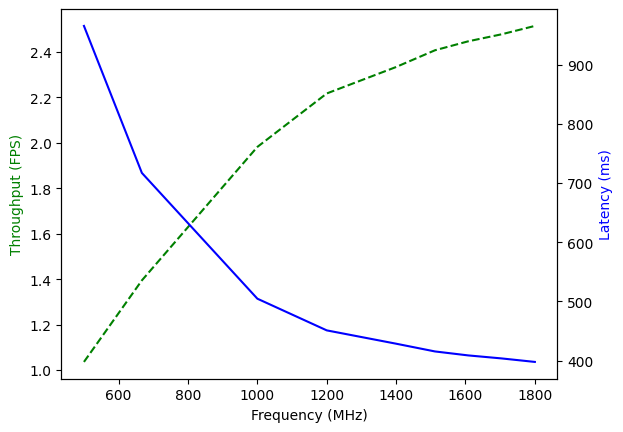
\includegraphics[width=0.85\linewidth]{figures/12.png}
    \caption{}
    \label{fig:exp1-little-freq_performance}
\end{figure}

Increasing Little CPU frequency improves throughput and reduces latency with diminishing returns at higher frequencies. Because power grows faster than FPS at high frequencies, we are interested in moderate (middle) frequencies for Little CPU.
\FloatBarrier

\par\vspace{\baselineskip}

\begin{figure}[!htbp]
    \centering
    \begin{subfigure}[b]{0.48\linewidth}
        \centering
        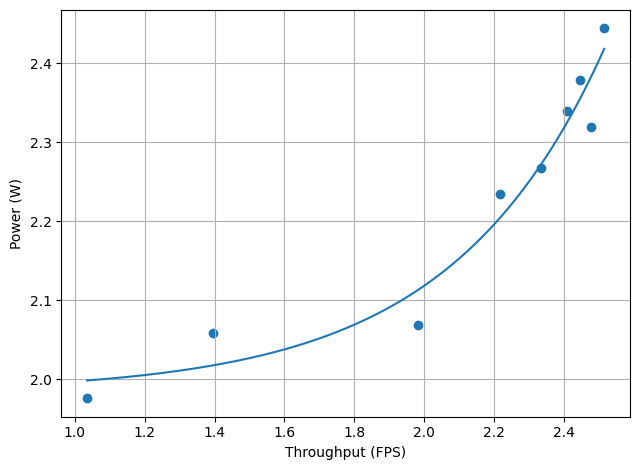
\includegraphics[width=\linewidth]{figures/13.png}
        \caption{}
    \end{subfigure}
    \hfill
    \begin{subfigure}[b]{0.48\linewidth}
        \centering
        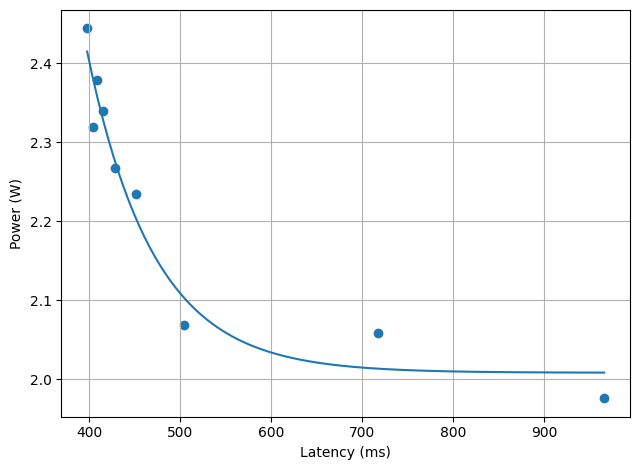
\includegraphics[width=\linewidth]{figures/14.png}
        \caption{}
    \end{subfigure}
    \caption{}
    \label{fig:exp1-little}
\end{figure}

The power–throughput plot shows a gradual trade-off: higher throughput requires higher power, but the slope remains relatively shallow compared to the Big CPU results. This indicates that the Little cluster offers moderate performance gains with relatively low additional power.

The power–latency relationship shows that reducing latency requires increased power, reflecting the typical energy–delay trade-off. At the lowest latencies, additional power produces smaller improvements, suggesting diminishing returns near the upper DVFS range. This motivates a governor policy that avoids the highest Little frequencies unless latency constraints demand them.
\FloatBarrier

\par\vspace{\baselineskip}

% ----- 2 ------
\textbf{2. Power-Performance graphs for AlexNet on Big CPU cluster at different frequencies.}\\

\begin{figure}[!htbp]
    \centering
    \begin{subfigure}[b]{0.48\linewidth}
        \centering
        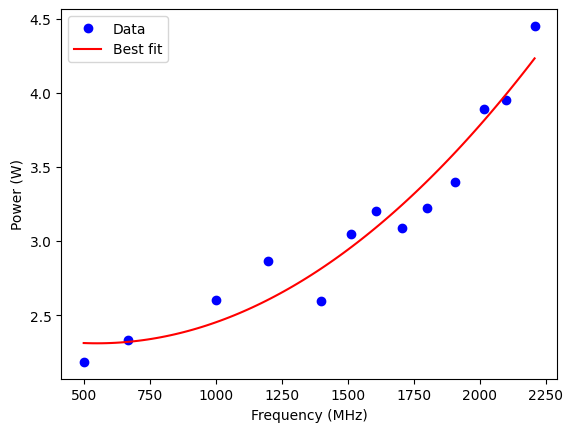
\includegraphics[width=\linewidth]{figures/21.png}
        \caption{}
    \end{subfigure}
    \hfill
    \begin{subfigure}[b]{0.48\linewidth}
        \centering
        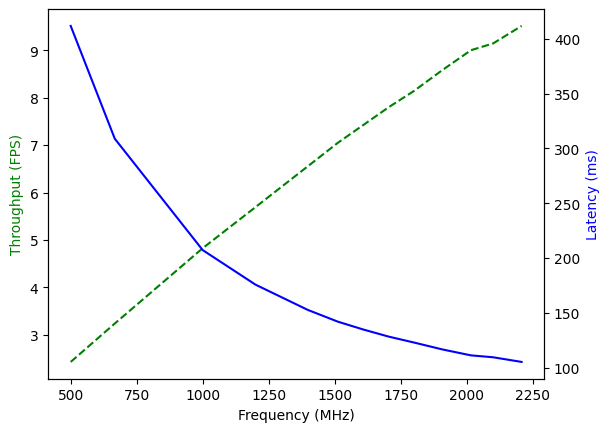
\includegraphics[width=\linewidth]{figures/22.png}
        \caption{}
    \end{subfigure}
    \caption{}
    \label{fig:exp2}
\end{figure}

Compared to the Little cluster, the Big cluster produces a much larger power swing across the frequency range, reflecting its high-performance microarchitecture and higher operating voltage requirements.
Performance increases significantly as Big CPU frequency increases, demonstrating that AlexNet inference is strongly accelerated by the Big cluster. However, the curves exhibit diminishing returns.
\FloatBarrier

\par\vspace{\baselineskip}

\begin{figure}[!htbp]
    \centering
    \begin{subfigure}[b]{0.48\linewidth}
        \centering
        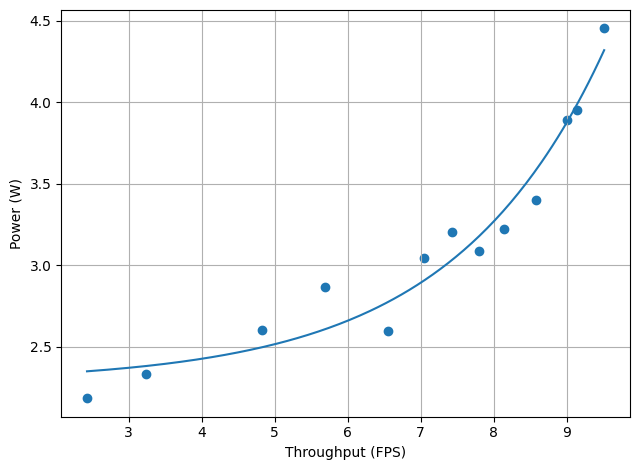
\includegraphics[width=\linewidth]{figures/23.png}
        \caption{}
    \end{subfigure}
    \hfill
    \begin{subfigure}[b]{0.48\linewidth}
        \centering
        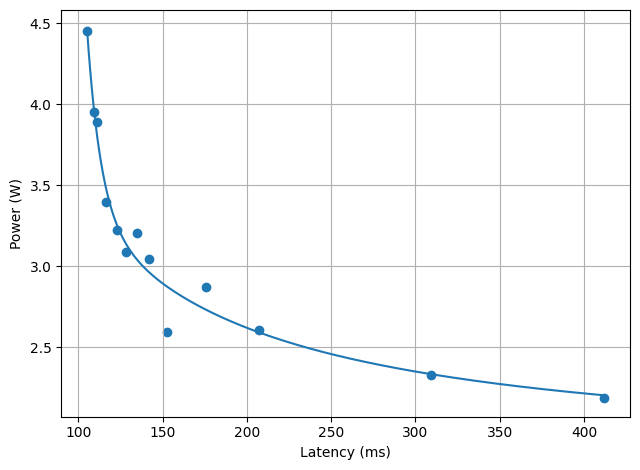
\includegraphics[width=\linewidth]{figures/24.png}
        \caption{}
    \end{subfigure}
    \caption{}
    \label{fig:exp22}
\end{figure}

The power–throughput and power–latency curves are steeper than for the Little cluster, indicating that the Big cluster is effective for meeting high throughput requirements but becomes power-inefficient at the highest performance points.
\FloatBarrier

\par\vspace{\baselineskip}

\begin{figure}[!t]
    \centering
    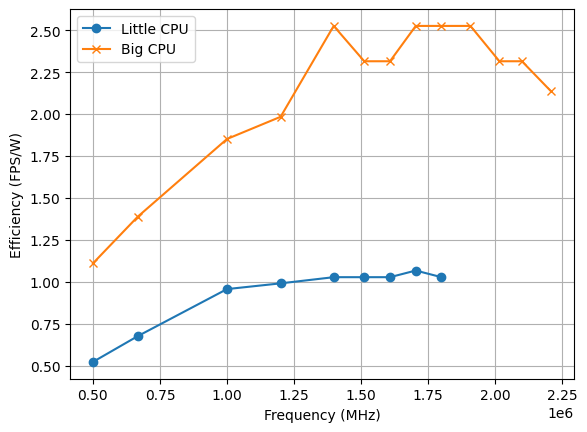
\includegraphics[width=0.85\linewidth]{figures/25.png}
    \caption{}
    \label{fig:exp12-efficiency-comparison}
\end{figure}

\FloatBarrier

\par\vspace{\baselineskip}

% ----- 3 ------
\textbf{3. Power-Performance graphs for AlexNet on GPU at different frequencies.}\\

\begin{figure}[!htbp]
    \centering
    \begin{subfigure}[b]{0.48\linewidth}
        \centering
        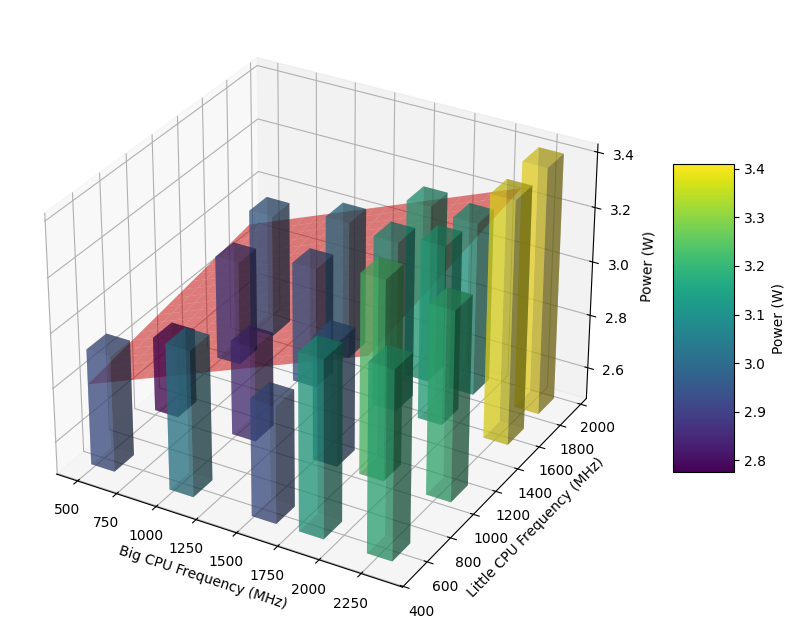
\includegraphics[width=\linewidth]{figures/31.png}
        \caption{}
        \label{fig:exp3-1}
    \end{subfigure}
    \hfill
    \begin{subfigure}[b]{0.48\linewidth}
        \centering
        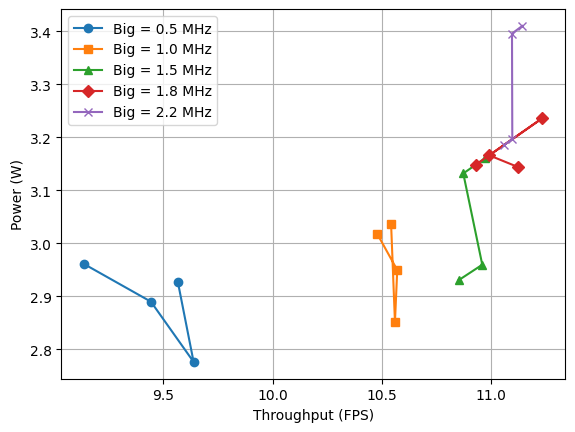
\includegraphics[width=\linewidth]{figures/32.png}
        \caption{}
        \label{fig:exp3-2}
    \end{subfigure}
    \caption{}
    \label{fig:exp3}
\end{figure}



\section{Conclusion [0.25 Points]} 

Discuss the potential concerns you may have about the characterization. Elaborate the potential pitfalls and how you would avoid it. Finally, explain how the characterization from this report will influence the design of your Governor.

\section{Mandatory Appendix}

Should the grade be divided equally between all team members: \textbf {Yes}. 

~

\noindent \textbf{Explain individual contributions (roles) of all team members.}


\section{Tips [Delete Me in Final Report]} 

\begin{itemize}

\item Experiments take time, so leave enough time for collecting results. Plan for re-running specific experiment instances for anomalous results or failed runs.

\item Since the total number of possible permutations and combinations for all partition orders, all partition points, and all DVFS frequencies is too large you cannot explore them all. So, carefully curate the experiments you want to run and explain your reasoning for the selection in the methodology.

\item Following good accessibility practices (for the color blind), your figure and graphs should be legible without colors. An ideal way to test this is that your report should be readable in gray-scale print, such as with extensive use of patterns.

\item This report tests your ability to collect data and think critically. It is not enough to present the results. You must also explain the results by reasoning about them to get full grade.

\end{itemize}

\end{document}